\subsection{Batch Processing of Files}

What should we do if we have more stacks that should be analyzed? Should we open each of the stack and execute the macro? A better idea is to automate the loading process also. For this, we modify and extend the code written in the previous section. The tasks are:

\begin{itemize}
\item task a: List files in a folder.
\item task b: Open a file, do analysis, save results and close the file. 
\item task c: Do this until all files are analyzed.
\end{itemize}
 
A very useful function for task a is \ilcom{getFileList(path)}.
\begin{indentCom}
\textbf{getFileList(directory)}\\
Returns an array containing the names of the files in the specified directory path. The names of subdirectories have a "/" appended.
\end{indentCom}
 
You need to set the path to the source image containing folder (directory). We learn this macro function in the following short macro. 

\lstinputlisting[morekeywords={*, getDirectory, getFileList}]{code/code22.ijm}

Run this macro and if you choose a folder in the sample image folder containing four stacks,  macro prints out texts in Log window. It should then look like figure \ref{fig:code22out}.
%figure 
\begin{figure}[htbp]
\begin{center}
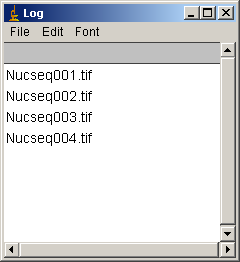
\includegraphics[scale=0.6]{fig/fig2521_FileBatchOUtput.png}
\caption{Output of code 22}
\label{fig:code22out}
\end{center}
\end{figure}

\begin{itemize}
\item Line 2: Asks the user to select a folder. Variable \ilcom{dir} is then stored with the full path to the folder. 
\item Line3 uses the \ilcom{getFileList} function, and reads out the file names as a string array and stored in List (array). 
\item Line 4 to 6 is a loop. \ilcom{list.length} returns the length of the list. In this way, all the contents are printed out in the window. 
We use this \ilcom{getFileList} function to process multiple files automatically. 
\end{itemize}

Let's modify code 22 so we can measure multiple stacks automatically. Code 23 (see below) works like this: You must first set two things: 

\begin{enumerate}
\item Full path to the destination folder where the results will be saved. 
Macro \ilcom{Set Directory to save Results}
\item Threshold level for the particle analysis. Macro \ilcom{set the threshold lower level}
\end{enumerate}

The first setting task is the same as you did in code 22. 
The second setting is done by manually opening a stack 
(may be the first one in the files) and manually setting the threshold as you like, 
then execute the second macro below. In both these settings, 
parameters will be saved in global variables and will be used in the main program. 

When you run the main macro (\ilcom{Multiple measurement}) 
after these two settings, the program asks you where the files are. 
As soon as you select a folder where files are contained, 
then processing and saving just proceeds automatically. 

\lstinputlisting[morekeywords={*, }]{code/code23_FileIO_02.ijm}

Now we have three macros and four global variables. 
\begin{itemize}
\item Line 3: global string variable for storing path to the source folder. 
\item Line 4: global string variable for storing path to the destination folder, where results will be saved. 
\item Line5 and 6: Global numerical variables for storing threshold upper and lower values. 

\item Macro \ilcom{Set Directory to save Results}: Line 9 to 12: First macro. This is used to set the path to the destination folder. The function is same as code 22.
 
\item Macro \ilcom{set the threshold lower level}: Line 14 to 20: 
This macro is for storing the lower value of the threshold in global variables, 
the values of which will be used in the main macro. You might have seen a similar code already: code 17, 
function for checking if the image is thresholded. 
Only difference is that in this code 23, 
lower threshold value is stored in the global variable defined in line 5. 
Upper value is not touched, kept to 255. 

\item Macro \ilcom{Multiple measurement}: Line 22 to 28: This is the main macro (third one in this macro set). 
Line 23 asks the user where the files are. 
This path to the source file is stored in the global variable defined in line 3. 
Then in line 24, a list of files contained in source folder is generated and stored in the array \ilcom{list}. 
From line 25 to 27 is a small for-loop, the number of loop is same as the length of the list. 
In this loop, name of file is passed one by one to the 
function \ilcom{NucAnalysis()} that does the actual analysis\ldots

\item function \ilcom{NucAnalysis(img\_filename)}: Line 30 to 51 is the core of analysis. 
\ilcom{img\_filename} is string variable for file names in the list array, given as argument. 
\begin{itemize}
\item Line 31: Using \ilcom{img\_filename},  the full path name is constructed by combining two strings. 
\item Line 32: A file is opened by \ilcom{open(path)} function. 
\begin{indentCom}
\textbf{open(path)}\\
Opens and displays a tiff, dicom, fits, pgm, jpeg, bmp, gif, lut, roi, or text file. 
Displays an error message and aborts the macro if the specified file is not in one of the supported formats, 
or if the file is not found. 
Displays a file open dialog box if path is an empty string or if there is no argument. 
Use the File>Open command with the command recorder running to generate calls to this function. 
With 1.41k or later, opens images specified by a URL.
\end{indentCom}
\item Line 33: After opening image, its \ilcom{ImageID} is stored in the variable \ilcom{sourceID}. 
\item Line 34, the image is thresholded according to the global variables for the lower and the upper values. 
\item Line 35: Title of the image, which actually is the file name, is retrieved and stored in the variable \ilcom{img\_title}. 
\item Line 38: The particle analysis is then applied to the image (Lines 34 to 37 are same as lines 14 to 17 in code 21). 
\item Line 38: Source image you opened from the hard disk is activated and then closed in line 39. 
Activation of the image by \ilcom{selectImage()} is required, 
because there is already a new stack (outline stack!), 
so that original stack is already behind. Therefore to close the original, 
one must activate the image by using \ilcom{selectImage()} function.  
\item After all these processing and measurement, results will be saved. 
Lines 42 to 45 saves the outline stack. Outline stack is also closed after saved (line 45). 
Line 47 to 50 is exactly same as the Result table saving you did in code 21 (lines 18 to 20). 
Line 49 is added, just for an additional information printout in Log window. 
\end{itemize}
\end{itemize}
